\documentclass{standalone}
%
\usepackage{tikz}
\usetikzlibrary{backgrounds,arrows.meta,shapes.callouts}
\usepackage{xcolor}
%
\definecolor{space}{HTML}{1F2C4E}
\definecolor{earth}{HTML}{0089FA}
\definecolor{dida}{HTML}{FFDE00}
\definecolor{title}{HTML}{FBA706}
\definecolor{galaxy}{HTML}{4278A4}
\definecolor{paper01}{HTML}{BE8A3F}
\definecolor{paper02}{HTML}{E5D09B}
%
\usepackage{fontspec}
\setmainfont{Open Dyslexic}
%
\title{Vite da raccontare}
\begin{document}
	\begin{tikzpicture}[background rectangle/.style={fill=white},show background rectangle,>={[inset=0,angle'=27]Stealth}]
		% title
		\draw [black,ultra thick,fill=title] (0,12.8) rectangle (30,16.8);
		\node at (15,14.8) {\textcolor{black}{\fontsize{75}{76}\selectfont Vite da raccontare}};
		% stripe
		\begin{scope}[shift={(0,12)}]
			\draw [fill=earth!50!white, thick] (14.5,0) rectangle (26.5,-149.5);
			\foreach \i in {0,1,...,11}
			{
				\draw [fill=white, thick] (14.75+\i,-0.5) rectangle (15.25+\i,-1);
			}
			%
			\foreach \j in {0,1,...,11}
			{
				\draw [fill=white, thick] (14.75+\j,-147.5) rectangle (15.25+\j,-148);
			}
		\end{scope}
		%
		% Ipazia
		%
		\begin{scope}[shift={(0,8)}]
			\draw [fill=white, thick] (3,0.8) rectangle (13,-10.8);
			\node at (8,-5) {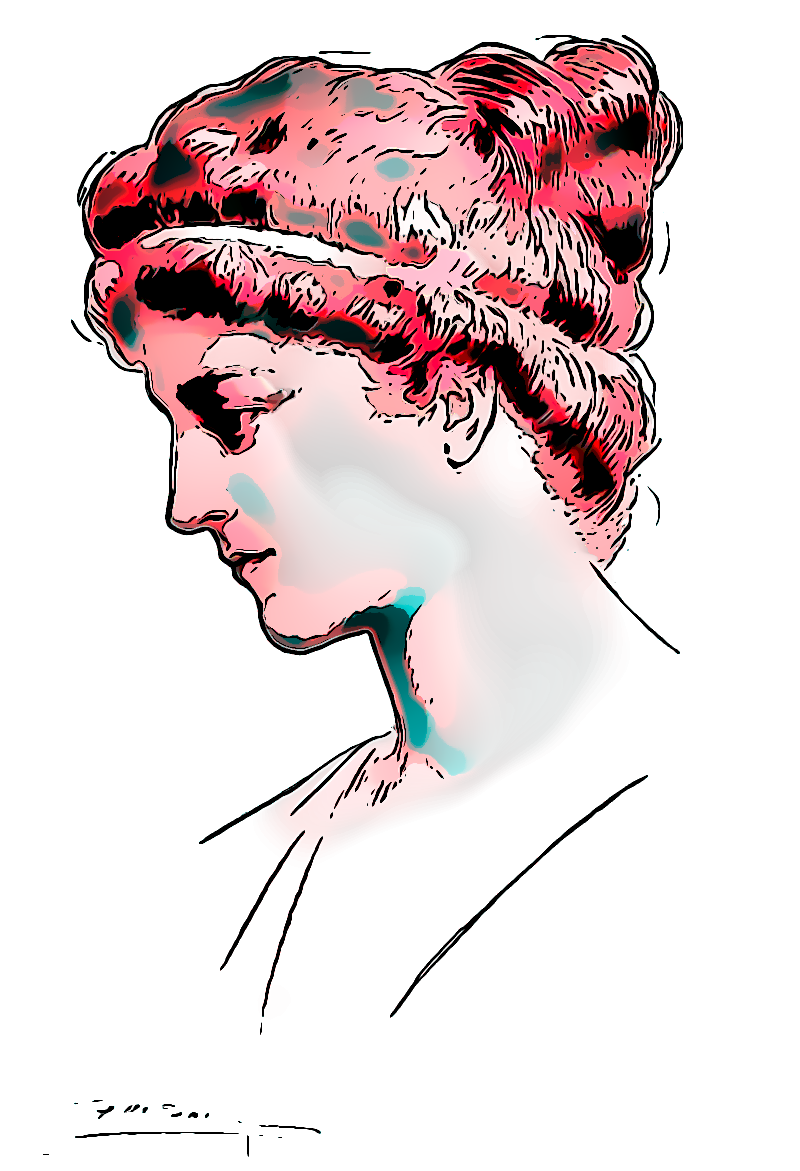
\includegraphics[width=8cm]{img/2025/ipazia}};
			%
			\draw [fill=galaxy, ultra thick] (3.5,-10.3) rectangle (12.5,-11.4);
			\node at (8,-10.9) {\textcolor{black}{\fontsize{18}{19}\selectfont Ipazia}};
			%
			\draw [fill=title, thick] (14,0.9) rectangle (27,1.8);
			\node (example-textwidth-2) [right, align=left, text width=12cm, color=black, font=\fontsize{18pt}{19pt}\selectfont] at (15,1.3) {\textbf{350-370}};
			%
			\node (example-textwidth-2) [right, align=left, text width=12cm, color=black, font=\fontsize{18pt}{19pt}\selectfont] at (15,-0.1) {Matematica e astronoma};
			%
			\draw [fill=dida, thick] (14,-1) rectangle (27,-20);
			\node (example-textwidth-2) [right, align=left, text width=11cm, color=black, font=\fontsize{18pt}{19pt}\selectfont] at (15,-10.5) {Figlia del filosofo e matematico \textbf{Teone}, gli succedete nell'insegnamento di tali materie. Dagli scritti di storici come \textbf{Esichio di Mileto}, ma anche grazie alla testimonianza diretta di allievi come \textbf{Sinesio}, sappiamo che Ipazia si interesso' di geometria e in particolare delle coniche, scrivendo un commentario sulle \emph{Coniche} di \textbf{Apollonio di Perga} e un altro sull'\emph{Arithmetica} di \textbf{Diofanto di Alessandria}, il padre dell'algebra noto soprattutto per le equazioni diofantee, quelle che possono essere risolte solo con numeri interi.\\Si e' interessata anche di astronomia poiché Sinesio ha confermato che i miglioramenti all'astrolabio che ha apportato discendono proprio dagli insegnamenti ricevuti in quel campo da Ipazia. Nella fisica, ha contribuito alla progettazione e costruzione di un idroscopio.};
			%
			\draw [fill=title, thick] (14,-20.8) rectangle (27,-21.8);
			\node (example-textwidth-2) [right, align=left, text width=12cm, color=black, font=\fontsize{18pt}{19pt}\selectfont] at (15,-21.3) {\textbf{Marzo 415}};
		\end{scope}
		%
		% Laura Bassi
		%
		\begin{scope}[shift={(0,-24.5)}]
			\foreach \i in {0,1,...,11}
			{
				\draw [fill=white, thick] (14.75+\i,9) rectangle (15.25+\i,9.5);
			}
			%
			\draw [fill=earth!50!white, thick] (3,6.5) rectangle (13,-7.6);
			\node at (8,-0.5) {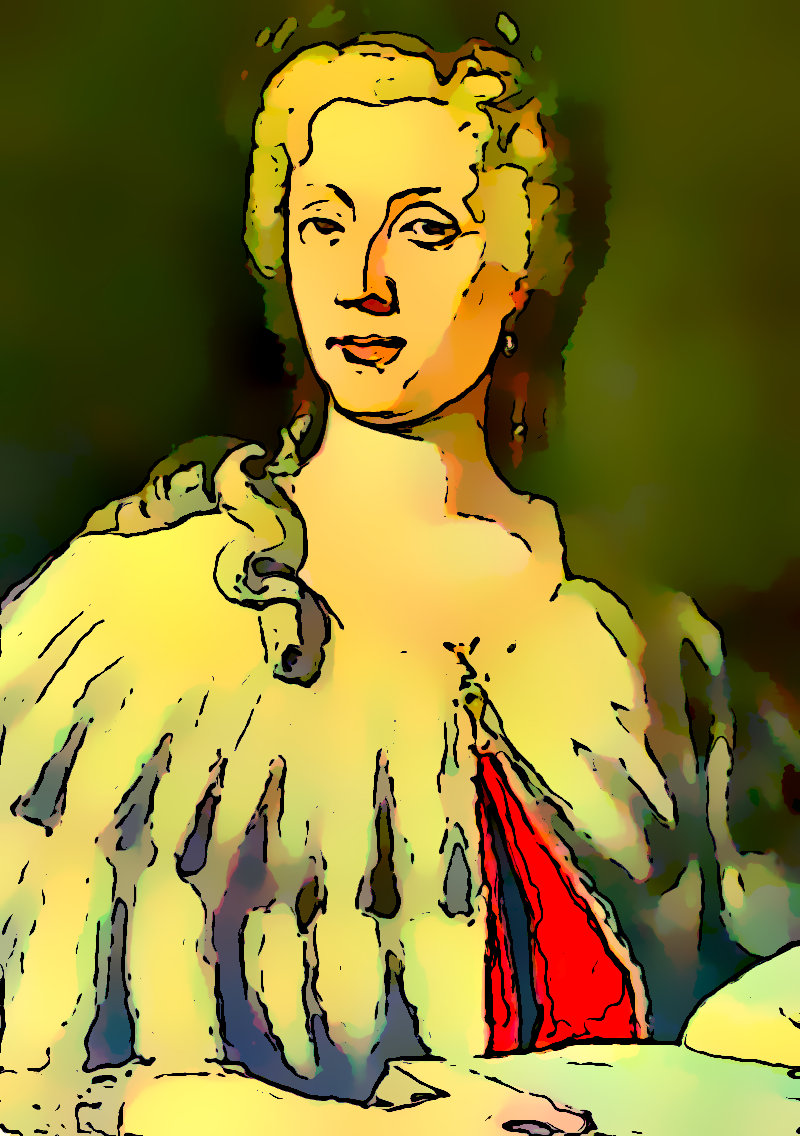
\includegraphics[width=9.96cm]{img/2025/laura_bassi}};
			%
			\draw [fill=galaxy, ultra thick] (4.6,-7) rectangle (11.4,-8);
			\node at (8,-7.5) {\textcolor{black}{\fontsize{18}{19}\selectfont Laura Bassi}};
			%
			\draw [fill=title, thick] (14,6.85) rectangle (27,7.75);
			\node (example-textwidth-2) [right, align=left, text width=12cm, color=black, font=\fontsize{18pt}{19pt}\selectfont] at (15,7.35) {\textbf{29-31 ottobre 1711}};
			%
			\node (example-textwidth-2) [right, align=left, text width=11cm, color=black, font=\fontsize{18pt}{19pt}\selectfont] at (15,5.5) {Matematica e fisica};
			%
			\draw [fill=dida, thick] (14,4.2) rectangle (27,-8.5);
			\node (example-textwidth-2) [right, align=left, text width=11cm, color=black, font=\fontsize{18pt}{19pt}\selectfont] at (15,-2.3) {Seconda donna al mondo ad aver ottenuto una laurea in filosofia, e' stata anche la prima ad aver ottenuto un dottorato in scienze. Venne istruita da Gaetano Tacconi, che convinse il padre Giuseppe a mandarla all'universita', ottenendo il titolo di Dottore in Filosofia il 12 maggio del 1732 a Bologna. Come per molti altri studiosi con lo stesso titolo, Laura Bassi mostra una certa vastità di interessi: l'acqua come elemento essenziale per la vita, l'anatomia, la letteratura (vennero pubblicate un paio di raccolte di sue poesie), ma soprattutto la fisica.};
			%
			\node (example-textwidth-2) [right, align=left, text width=11cm, color=black, font=\fontsize{18pt}{19pt}\selectfont] at (15,-18.7) {In questo campo, oltre all'impegno nel portare e diffondere in Italia le leggi scoperte da \textbf{Isaac Newton}, anche grazie alla realizzazione di esperimenti di fisica di base, realizzò anche esperimenti nel campo dell'elettricità, ispirata al lavoro d'oltreoceano di \textbf{Benjamin Franklin}. In particolare in quest'ultimo campo diede inizio a una piccola scuola che proseguì con \textbf{Luigi Galvani}, che fu suo allievo. Ebbe una vasta corrispondenza con molti intellettuali e scienziati dell'epoca, tra cui si contano \textbf{Ruggero Boscovich}, \textbf{Lazzaro Spallanzani}, \textbf{Alessandro Volta}. Il suo credito, poi, era tale che, quando nel 1772 \textbf{Paolo Balbi}, titolare della cattedra di fisica a Bologna, mori' improvvisamente, l'Universita' decise di conferire proprio a Laura Bassi la cattedra: era il 1776 e non solo Laura diventava la titolare di una prestigiosa cattedra, ma aveva il marito, \textbf{Giuseppe Veratti}, come assistente!};
			%
			\draw [fill=title, thick] (14,-28.8) rectangle (27,-29.8);
			\node (example-textwidth-2) [right, align=left, text width=12cm, color=black, font=\fontsize{18pt}{19pt}\selectfont] at (15,-29.2) {\textbf{20 febbraio 1778}};
		\end{scope}
		%
		% Agnes Giberne
		%
		\begin{scope}[shift={(0,-64.7)}]
			\foreach \i in {0,1,...,11}
			{
				\draw [fill=white, thick] (14.75+\i,8.8) rectangle (15.25+\i,9.3);
			}
			%
			\draw [thick] (3,6.5) rectangle (13,-9);
			\node at (8,-1.3) {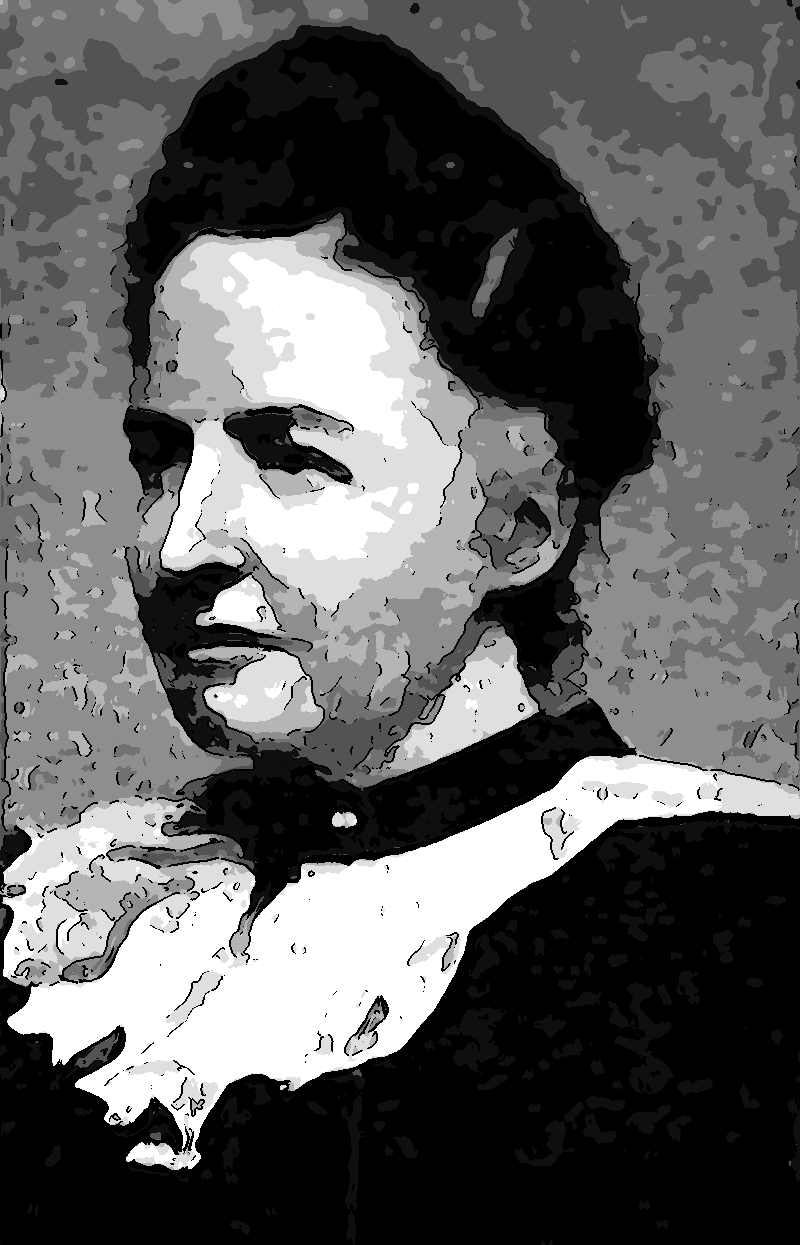
\includegraphics[width=10cm]{img/2025/agnes_giberne}};
			%
			\draw [fill=galaxy, ultra thick] (5.3,-8.6) rectangle (10.7,-9.6);
			\node at (8,-9.1) {\textcolor{black}{\fontsize{18}{19}\selectfont Agnes Giberne}};
			%
			\draw [fill=title, thick] (14,6.55) rectangle (27,7.45);
			\node (example-textwidth-2) [right, align=left, text width=12cm, color=black, font=\fontsize{18pt}{19pt}\selectfont] at (15,6.95) {\textbf{19 novembre 1845}};
			%
			\node (example-textwidth-2) [right, align=left, text width=10cm, color=black, font=\fontsize{18pt}{19pt}\selectfont] at (15,5.6) {Scrittrice e divulgatrice scientifica};
			%
			\draw [fill=dida, thick] (14,4.5) rectangle (27,-6.1);
			\node (example-textwidth-2) [right, align=left, text width=10cm, color=black, font=\fontsize{18pt}{19pt}\selectfont] at (15,-0.8) {Istruita in casa, venne introdotta alla letteratura dalla madre, \textbf{Lydia Mary Wilson}, e si interesso' di scienza grazie al padre, \textbf{Charles Giberne}, capitano della \emph{Bengal Native Infantry}. Il suo primo libro, un romanzo per l'infanzia, \emph{A Visit to Aunt Agnes}, venne pubblicato nel 1864. Oltre ai libri per bambini, scrisse anche alcuni romanzi storici, ma e' nota soprattutto per i suoi testi di divulgazione scientifica.};
			%
			\node (example-textwidth-2) [right, align=left, text width=11cm, color=black, font=\fontsize{18pt}{19pt}\selectfont] at (15,-13) {Nei suoi libri ha affrontato discipline come la geologia, la fisica, l'idrologia, la meteorologia, la storia naturale e molte altre. Essendo, pero', un'astronoma dilettante, ha dedicato un'ampia porzione della sua produzione saggistica all'astronomia. Non a caso il suo primo libro divulgativo, pubblicato nel 1879, aveva come titolo \emph{Sun, Moon and Stars: Astronomy for Beginners}. Con l'introduzione di \textbf{Charles Pritchard}, scritta su sua iniziativa, il libro fu un grande successo, diventando il primo di una lunga serie. A proposito di questo esordio, \emph{The Graphic}, settimanale britannico illustrato, ebbe modo di scrivere:};			
			%
			\shade [bottom color=paper02,top color=paper01] (14,-20.3) rectangle (27,-23.9);
			\draw [thick] (14,-20.3) rectangle (27,-23.9);
			\node (example-textwidth-2) [right, align=left, text width=11cm, color=black, font=\fontsize{18pt}{19pt}\selectfont] at (15,-22) {Come introduzione a una scienza, non potrebbe essere piu' attraente, ed e' il miglior libro del genere che abbiamo mai letto.};
			%
			\node (example-textwidth-2) [right, align=left, text width=11cm, color=black, font=\fontsize{18pt}{19pt}\selectfont] at (15,-27.2) {Nel 1890 ha contribuito a fondare la \emph{British Astronomical Association}. Successivamente, nel 1899, l'astronoma \textbf{Elizabeth Brown}, che aveva contribuito a fondare la BAA insieme con Agnes Giberne, divenne direttrice dalla \emph{Solar Section} dell'associazione.};
			%
			\draw [fill=title, thick] (14,-30.5) rectangle (27,-31.4);
			\node (example-textwidth-2) [right, align=left, text width=12cm, color=black, font=\fontsize{18pt}{19pt}\selectfont] at (15,-31) {\textbf{20 agosto 1939}};
		\end{scope}
		%
		% Jocelyn Bell
		%
		\begin{scope}[shift={(0,-103.5)}]
			\foreach \i in {0,1,...,11}
			{
				\draw [fill=white, thick] (14.75+\i,6.4) rectangle (15.25+\i,5.9);
			}
			%
			\draw [thick] (3,3.95) rectangle (13,-11.75);
			\node at (8,-3.9) {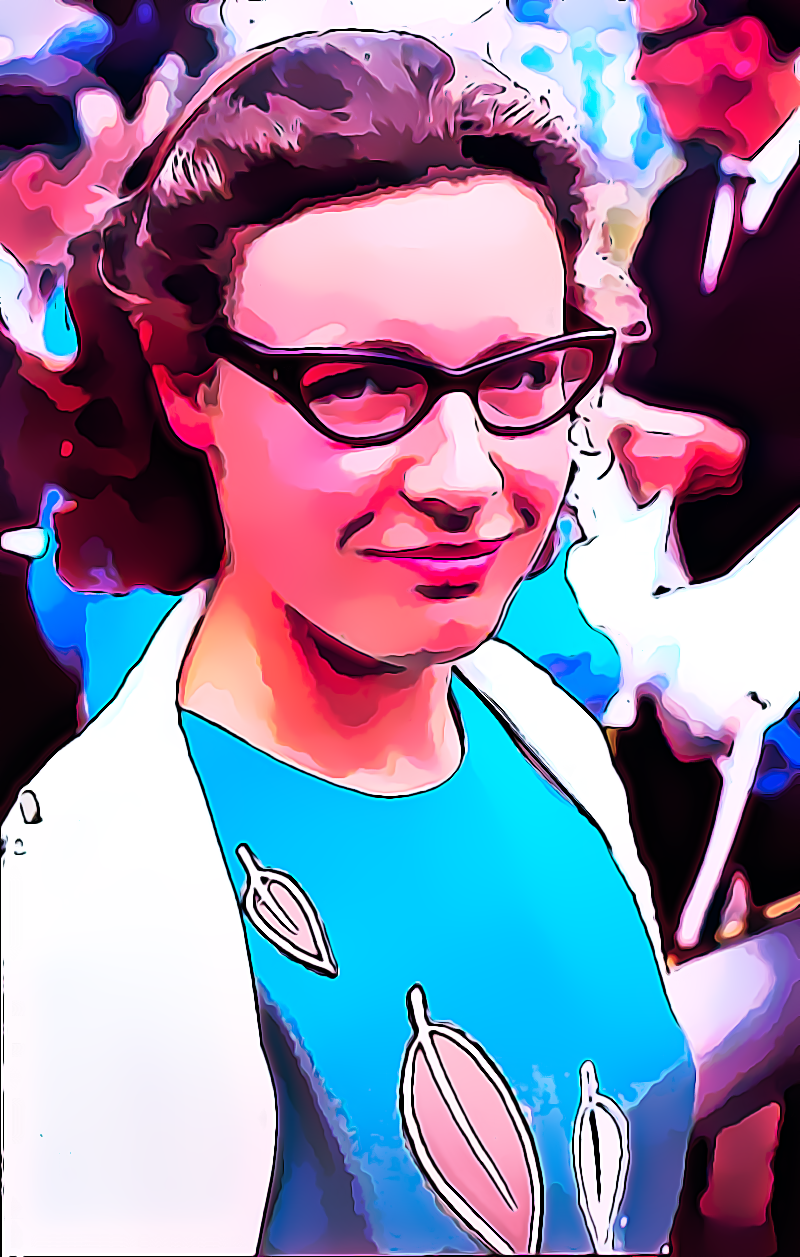
\includegraphics[width=10cm]{img/2025/jocelyn_bell}};
			%
			\draw [fill=galaxy, ultra thick] (5.2,-11.3) rectangle (10.8,-12.3);
			\node at (8,-11.8) {\textcolor{black}{\fontsize{18}{19}\selectfont Jocelyn Bell}};
			%
			\draw [fill=title, thick] (14,3.95) rectangle (27,4.85);
			\node (example-textwidth-2) [right, align=left, text width=12cm, color=black, font=\fontsize{18pt}{19pt}\selectfont] at (15,4.35) {\textbf{15 luglio 1943}};
			%
			\node (example-textwidth-2) [right, align=left, text width=10cm, color=black, font=\fontsize{18pt}{19pt}\selectfont] at (15,3) {Astronoma};
			%
			\draw [fill=dida,thick] (14,2.2) rectangle (27,-8);
			\node (example-textwidth-2) [right, align=left, text width=11cm, color=black, font=\fontsize{18pt}{19pt}\selectfont] at (14.8,-2.9) {Nel luglio del 1967 era a Cambridge per il suo dottorato in astronomia quando si imbatte' in alcuni segnali radio anomali per via della loro grande regolarita'. Jocelyn e il suo supervisore \textbf{Antony Hewish} iniziarono a esaminare dati e articoli arrivando alla conclusione che questo segnale poteva essere generato solo da una stella superdensa in rapida rotazione su se stessa: era la prima osservazione di una \emph{pulsar}.};
			%
			\node (example-textwidth-2) [right, align=left, text width=11cm, color=black, font=\fontsize{18pt}{19pt}\selectfont] at (15,-14.4) {La scoperta delle \emph{pulsar} frutto' a Hewish il Premio Nobel per la fisica nel 1974, ottenuto insieme con \textbf{Martin Ryle}, quest'ultimo per il suo contributo allo sviluppo dell'astronomia radio. Jocelyn, invece, non ottenne alcun riconoscimento da parte dell'Accademia Svedese, lei che era stata la prima a osservare quel segnale e il cui nome era il secondo nell'articolo uscito con l'annuncio della scoperta. Eppure il mancato Premio Nobel, non ha mai scoraggiato l'astronoma, che ne ha anzi trovato l'elemento piu' squisitamente positivo:};
			%
			\shade [bottom color=paper02,top color=paper01] (14,-21.2) rectangle (27,-30.6);
			\draw [thick] (14,-21.2) rectangle (27,-30.6);
			\node (example-textwidth-2) [right, align=left, text width=11cm, color=black, font=\fontsize{18pt}{19pt}\selectfont] at (15,-25.8) {Puoi realmente fare molto bene senza ottenere un premio Nobel, e ho ricevuto molti premi, e molti onori, e molti riconoscimenti, che in realta' penso di essermi divertita molto di piu' che se avessi ottenuto un premio Nobel - che e' un piccolo fuoco di paglia: puoi riceverlo, avere una settimana divertente, ed e' tutto li', e nessuno ti da altro dopo, perche' sentono di non poterlo eguagliare.};
			%
			%\draw [fill=title, thick] (14,-20.6) rectangle (27,-21.6);
			%\node (example-textwidth-2) [right, align=left, text width=12cm, color=black, font=\fontsize{18pt}{19pt}\selectfont] at (15,-21.1) {\textbf{1836}};
		\end{scope}
		% image credits
		\begin{scope}[shift={(0,-139)}]
			\draw [fill=space,thick] (2,1) rectangle (28,-1);
			%
			\node (example-textwidth-2) [right, align=left, text width=25cm, color=white, font=\fontsize{18pt}{19pt}\selectfont] at (2.5,0) {Le immagini sono tratte da Wikipedia o da Project Gutenberg e poi rielaborate graficamente usando il filtro G'MIC-Qt di Gimp.};
		\end{scope}
		%
		\begin{scope}[shift={(0,-141)}]
			\node at (27,0) () {
\includegraphics[width=3.7cm]{licenza}};
			\node (example-textwidth-2) [right, align=left, text width=14cm, color=black, font=\fontsize{14pt}{15pt}\selectfont] at (12.5,-0.1) {Testo e grafica: @ulaulaman - Gianluigi Filippelli};
		\end{scope}
	\end{tikzpicture}
\end{document}
